\begin{block}{Spatially Distributed Temperature Extremes}
    It is difficult for a single index to capture supply-side risk given complex interlinkages between natural gas, electric, and other systems.
    We thus estimate the exceedance probability of the February 2021 temperatures at each grid cell separately to shed light on the degree to which cold experienced by installations across the region was unprecedented.
    \begin{framed}
        \begin{figure}
            \centering
            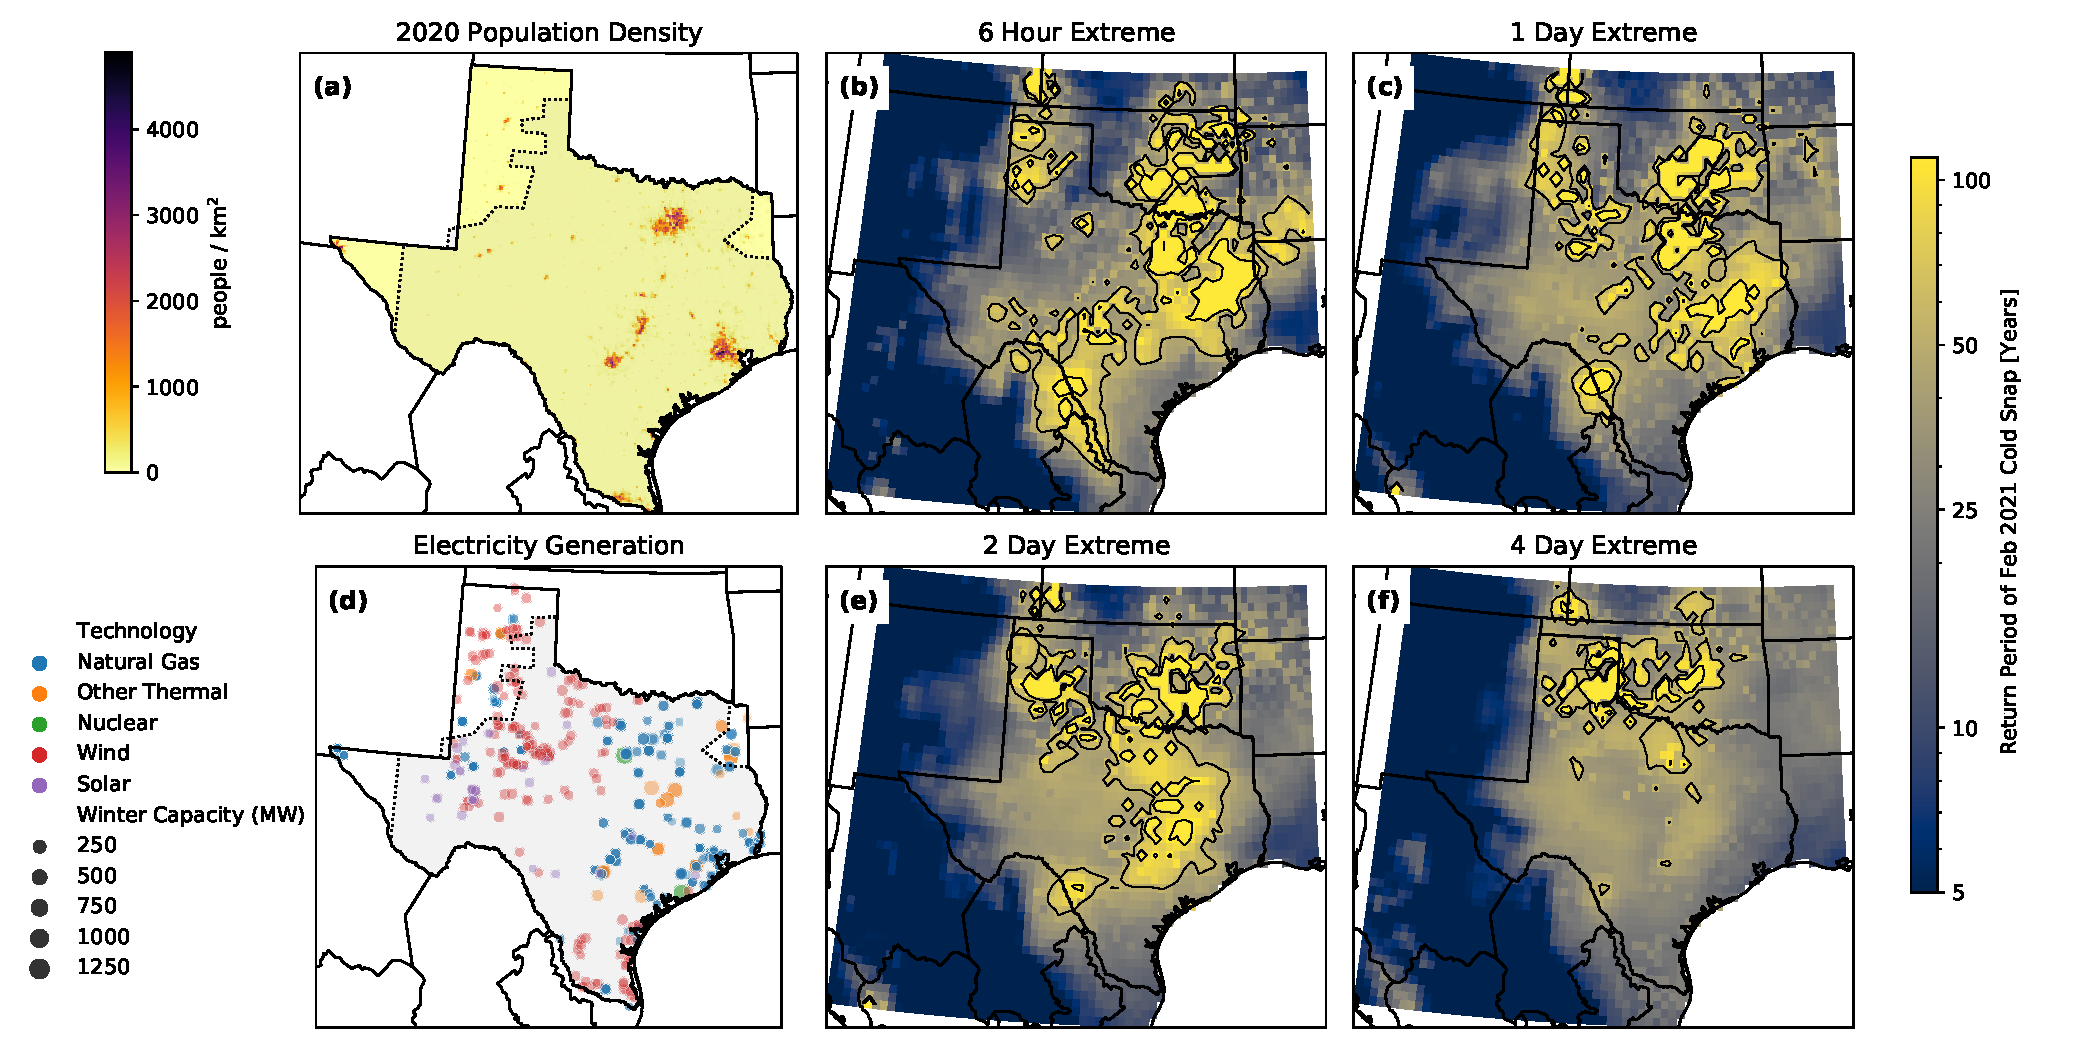
\includegraphics[width=\textwidth]{local_rt_era5.pdf}
            \caption{
                \textbf{Although the exceedance probability of February 2021's cold was less than 1/100 for some locations, for most it was between 1/25 and 1/50.}
                Return periods are calculated separately for each cell.
                (a): estimates of 2020 population density \cite{ciesin_gpwv4:2016}.
                (d): energy generation facilities in Texas \cite{useia_generators:2021}.
                (b,c,e,f): local return periods for 6 hour, 1 day, 2 day, and 4 day durations, respectively.
                Contours enclose regions that recorded 50 and 100 year return levels.
                The gray region in panels (a) and (d) shows boundaries of the Texas Interconnection \cite{useia_regions:2021}.
            }\label{fig:local_era5}
        \end{figure}
    \end{framed}
\end{block}